\documentclass[12pt]{article}

\usepackage{polski}
\usepackage[utf8]{inputenc}
\usepackage{graphicx}
\usepackage{xcolor}
\usepackage{float}
\usepackage{caption}
\usepackage{array}
\usepackage{pbox}
\usepackage{tikz}
\usetikzlibrary{arrows}
\usepackage{amsmath}
\usepackage{hyperref}

\newcommand\tab[1][1cm]{\hspace*{#1}}

\title{Dokumentacja projektowa}
\date{2018-03-18}
\author{Jędrzej Kozal}

\begin{document}
\bibliographystyle{plabbrv}

\begin{titlepage}
	\centering
	
\includegraphics[width=0.25\textwidth]{logo_pol_wroclaw.png}\par\vspace{1cm}
	{\scshape\LARGE Politechnika Wrocławska \par}
	\vspace{1cm}
	{\scshape\Large Wybrane zagadnienia projektowania obiektowego\par}
	\vspace{1.5cm}
	{\huge\bfseries Platforma testowa dla algorytmów uczenia nadzorowanego \par}
	\vspace{2cm}
	{\Large\itshape Filip Guzy\par}
	{\Large\itshape Jędrzej Kozal\par}
	{\Large\itshape Marcin Łokietko\par}

	\vfill
	prowadzący\par
	Dr inż.~Jacek \textsc{Cichosz}

	\vfill

% Bottom of the page
	{\large \today\par}
\end{titlepage}

\tableofcontents
\newpage


\section{Streszczenie}
%Streszczenie, w którym określamy cel projektu. Na przykład, obiektowy model topologii sieci komputerowej może służyć do wizualizacji rozmieszczenia jej węzłów, planowania routingu, itd. Staramy się umieścić nasz system w pewnej ogólnej klasie, np. typu klient–serwer, z bazą danych, sterowany zdarzeniowo, czasu rzeczywistego lub inny. Czy nasz system jest samodzielną aplikacją, fragmentem biblioteki klas, zrębu (ang. framework), komponentu, itp.? 
%Jakie techniki zostały zastosowane (rodzaje dziedziczenia, składania, wymienić zastosowane wzorce projektowe). Wymienić sugerowane języki implementacji, środowiska i proponowane narzędzia. Streszczenie powinno być krótkie (punkty, hasła).

\subsection{Założenia projektu}

Platforma testowa dla algorytmów uczenia maszynowego jest frameworkiem mającym umożliwiać przeprowadzanie eksperymentów w elastyczny i prosty sposób. W założeniu framework ma pozwalać na skonfigurowanie eksperymentu oraz zebranie wszystkich wyników potrzebnych do określenie skuteczności algorytmu, wygenerowania dokumentacji i zapisu przebiegu. Konstrukcja frameworka ma pozwalać na łatwą integrację w środowisku Continuous Integration.

W trakcie projektowania systemu uwzględniono wysokopoziomowy opis całej aplikacji z podziałem na komponenty oraz niskopoziomowy opis z wyszczególnieniem klas i ich odpowiedzialności.

\subsection{Wykorzystane wzorce i narzędzia}

W trakcie prac nad projektem wykorzystano następujące wzorce projektowe:

\begin{itemize}
	\item Budowniczy,
	\item Adapter,
	\item Strategia,
	\item Kompozyt,
	\item Polecenie,
	\item Mediator.
\end{itemize}

Dokładny opis wykorzystanych wzorców można znaleźć w \cite{gang-of-four}.

Rozważano najpopularniejsze języki wspierające obiektowy paradygmat programowania tj. Java, C++, Python lub C\#. W dalszej części pracy zawarto szczegółową analizę dostępnych języków implementacji wraz z umotywowaniem podjętego wyboru.

TO DO: Dopisać wykorzystane narzędzia.


\section{Wstępny opis słowny}
% 2. Wstępny opis słowny dotyczy tego co system robi, a nie jak. Jest to wyjściowy model werbalny działania systemu, może być on wynikiem wywiadu z potencjalnymi użytkownikami. Zwracamy uwagę na ważne pojęcia, które pojawiły się w opisie, staramy się je ściślej zdefiniować i usystematyzować. Pojęcia te (głównie rzeczowniki) można przedstawić w formie słownika (glosariusza).

Celem zaprojektowanego systemu jest badanie skuteczności wybranych algorytmów \textbf{uczenia nadzorowanego} - rodziny metod należących do dziedziny \textbf{uczenia maszynowego}.
Framework wspiera zarówno metody \textbf{klasyfikacji}, jak i \textbf{regresji}. Jakość analizowanych metod określana jest za pomocą wybranych przez użytkownika \textbf{miar}. W zależności od konfiguracji eksperymentu badania przeprowadzane są z wykorzystaniem klasycznej metody \textbf{holdout} lub \textbf{walidacji krzyżowej} o wybranych parametrach.

Testy wykonywane są na sparametryzowanej przez użytkownika bazie danych, która może podlegać przeprowadzanej przez framework analizie, obejmującej na przykład wykrywanie jej niezbalansowania.

Aplikacja umożliwia porównanie algorytmów na drodze \textbf{statystycznej analizy wyników}.
Wszystkie rezultaty eksperymentów reprezentowane są w graficznej postaci.


\section{Słownik pojęć z dziedziny problemu}
%3. Słownik pojęć z dziedziny problemu ułatwia systematykę pojęć z dziedziny problemu, który rozwiązujemy. Przedstawia wyłowione z opisu słownego określenia, które przełożą się następnie na składniki oprogramowania takie jak np. klasy. Zdarza się, że do reprezentacji niektórych pojęć potrzeba kilku klas. Często w systemie pojawią się także klasy nie odpowiadające bezpośrednio terminom w słowniku, a dotyczące dziedziny implementacji.

Poniżej przedstawiono definicje wyszczególnionych pojęć z poprzedniej sekcji pracy:

\begin{itemize}
	\item 
	\textbf{Uczenie nadzorowane} -- zadanie \textbf{uczenia maszynowego}, w którym dane uczące zawierają wektory wejściowe algorytmu wraz z jego oczekiwanym wyjściem\cite{Bishop2006}. 
	
	\item 
	\textbf{Uczenie maszynowe} -- dziedzina, której celem jest optymalizacja parametrów algorytmu na podstawie posiadanych danych. Ocena jakości algorytmów dokonywana jest z wykorzystaniem przyjętej funkcji strat.
	\cite{Alpaydin2014}
	
	\item 
	\textbf{Zadanie klasyfikacji} -- przypisanie wejściowego wektora do jednego z elementów skończonego zbioru kategorii\cite{Bishop2006}. 
	
	\item 
	\textbf{Zadanie regresji} -- zadanie uczenia maszynowego, w którym oczekiwanym wyjściem algorytmu dla danego wektora wejściowego jest wartość ciągła\cite{Bishop2006}.
	
	\item 
	\textbf{Miara jakości algorytmu} -- metryka służąca ocenie działania algorytmu przy przetwarzaniu danych, które nie zostały wykorzystane podczas uczenia.
	
	\item 
	\textbf{Holdout} -- metoda wyznaczania zbiorów treningowego i testowego poprzez jednokrotny podział danych uczących na dwie części.
	
	\item 
	\textbf{Walidacja krzyżowa} -- alternatywna do podejścia \textbf{holdout} metoda polegająca na wielokrotnym podziale dostępnych danych na zbiory treningowy i testowy, na których osobno uczony i testowany jest badany algorytm\cite{Alpaydin2014}.

	\item 
	\textbf{Statystyczna analiza miar jakości algorytmów} -- przetwarzanie wartości miar skuteczności algorytmów, którego celem jest określenie, czy różnice jakości metod są istotne statystycznie\cite{Dietterich1998}.
	
\end{itemize}




\section{Analiza wymagań użytkownika}
%4. Analiza wymagań użytkownika, w której można zastosować poznane w ramach przedmiotu ”inżynieria oprogramowania” przypadki użycia (ang. use case). Ważne jest zrozumienie jak system jest widziany z punktu widzenia użytkownika. Można przedstawić w tym punkcie główny scenariusz działania oraz najciekawsze scenariusze poboczne (czyli tzw. nietypowe sytuacje).

Projekt ma charakter frameworku, którego głównymi użytkownikami będą inni programiści. Z tego powodu projekt aplikacji powinien być prosty i intuicyjny w wykorzystaniu. W przypadku realizowanego tematu może być to trudne do osiągnięcia ze względu na złożoność omawianych zagadnień. W tej sekcji pracy przedstawiono analizę przypadków użycia frameworku, które stanowią podstawę projektu API dostępnego dla użykownika.

\subsection{Podstawowe przypadki użycia}

Przewiduje się następujące przypadki użycia:

\begin{itemize}
	\item konfiguracja i przeprowadzenie eksperymentu z wykorzystaniem:
	\begin{itemize}
		\item dostarczonych algorytmów:
		\begin{itemize}
			\item klasyfikacji
			\item regresji		
		\end{itemize}
		\item metod uzyskiwania wyników:
		\begin{itemize}
			\item K-krotnej walidacji krzyżowej
			\item 5-2 walidacji krzyżowej
			\item metody "HoldOut"
		\end{itemize}
		\item wybranych metryk:
		\begin{itemize}
			\item dokładności
			\item czułości
			\item swoistość
			\item krzywej ROC
			\item pola pod krzywą ROC
			\item F1-score
			\item G-mean
			\item błędu średniokwadratowego
		\end{itemize}
		\item funkcjonalności do analizy wyników:
		\begin{itemize}
			\item zapisywania wyników
			\item generowania i zapisywania wyników
			\item testowania hipotez i przeprowadzania testów post-hoc
		\end{itemize}
	\end{itemize}
	\item przeprowadzania analizy zbioru uczącego:
	\begin{itemize}
		\item Analizy niezbalansowania zbioru
		\item Estymacji VC-dim
	\end{itemize}
\end{itemize}

\subsection{Nietypowe przypadki}

Najczęstszym źródłem nietypowych sytuacji mogą być przypadki w których użytkownik nie poda właściwych danych, co może skutkować wystąpieniem wyjątków w modułach konfigurujących pracę systemu. Przykładowo użytkownik dla algorytmu klasyfikacji może podać metrykę przewidzianą dla regresji. Innym przypadkiem z tej kategorii może być podanie jako argumentu referencji do NullPointera. Są to problemy, które powinny być rozwiązywane przez moduły konfigurujące pracę systemu, przez komunikowanie użytkownika o błędnej konfiguracji.
 
Wyjątkowa sytuacja, która nie może być wykryta na poziomie konfiguracji systemu to podanie zbioru uczącego zawierającego mniej próbek, niż jest to wymagane przez algorytmy walidacji krzyżowej. Przykładowo dla 10-krotnej walidacji musi zostać utworzone 10 podzbiorów datasetu co oznacza, że zbiór uczący musi posiadać co najmniej 10 próbek. Sprawdzanie tego typu scenariuszy musi odbywać się na poziomie klasy realizującej walidację krzyżową. Próba zabezpieczenia się przed takimi sytuacjami w innym miejscu powodowałaby mieszanie informacji o charakterze i odpowiedzialności poszczególnych komponentów i łamanie dobrych zasad projektowania.

\subsection{Podstawowe założenia systemu obsługi błędów}

Zgodnie z dobrymi zasadami programowania obiektowego \cite{clean-code} przyjęto, że framework będzie komunikował użytkownika o wystąpieniu błędu przez zgłoszenie odpowiedniego wyjątku. Każdy wyjątek powinien mieć typ zdefiniowany w frameworku - poleca się unikanie ogólnych typów wyjątków. Ponadto wyjątki powinny zawierać wszystkie niezbędne informacje o kontekście i lokalizacji błędu, co powinno ułatwić korzystanie z frameworku. Przyjęto takie rozwiązanie ponieważ większość błędów omówiona w poprzedniej subsekcji pracy może wynikać z nieprawidłowej konfiguracji przez użytkownika. 

Istnieją alternatywy dla wybranego rozwiązania jak np. modyfikacja interfejsów, tak aby zwracały informacje o tym, czy dana operacja zakończyła się sukcesem lub rozwiązania specyficzne dla wybranych języków programowania np. system obsługi błędów w Go, gdzie każda funkcja oprócz rezultatu zwraca obiekt informujący o błędzie. Rozwiązania te zostały odrzucone ponieważ mają zły wpływ na kod. Główną korzyścią stosowania wyjątków jest oddzielenie normalnej logiki aplikacji od kodu obsługującego błędy, co ułatwia konserwację i rozwijanie kodu. 

\section{Modele systemu z różnych perspektyw}
%5. Modele systemu z różnych perspektyw to najważniejsza część projektu, w której posiłkujemy się językiem UML do przedstawienia struktury i zachowania naszego systemu. Podstawowym diagramem do opisu struktury jest diagram klas, natomiast zachowanie systemu można zobrazować diagramem sekwencji. W razie potrzeby wykonujemy inne rysunki wyjaśniające nasze idee i koncepcje. Nie boimy się przedstawiać alternatywnych rozwiązań jakiegoś problemu i analizować konsekwencje. Rysunkom muszą towarzyszyć słowne komentarze i wyjaśnienia, dopiero te dwa elementy (grafika + tekst) ułatwiają zrozumienie intencji autora. Wszelkie decyzje projektowe powinny być uzasadnione. Właściwe projektowanie można zacząć od naszkicowania współpracy obiektów w celu realizacji scenariuszy działania systemu opisanych na etapie analizy. W dalszej kolejności przypisujemy obiekty do poszczególnych klas. Wtedy często może się okazać, że potrzebnych jest więcej klas niż założyliśmy wstępnie. Należy zwrócić uwagę aby modele systemu z różnych perspektyw były spójne.

W niniejszej sekcji pracy przedstawiono wysokopoziomowy opis architektury zwierający informacje o wyszczególnionych komponentach, zakresie ich odpowiedzialności oraz sposobie komunikacji. Zawarto tu również bardziej szczegółowe modele poszczególnych komponentów z uwzględnieniem diagramów klas i diagramów przepływu.

\subsection{Wysokopoziomowa koncepcja architektury aplikacji}

We frameworku wyszczególniono następujące komponenty:

\begin{itemize}
	\item TestPlatform,
	\item Dataset,
	\item Validation,
	\item Algorithm,
	\item ResultAnalyser.
\end{itemize}


\begin{figure}
\centering
	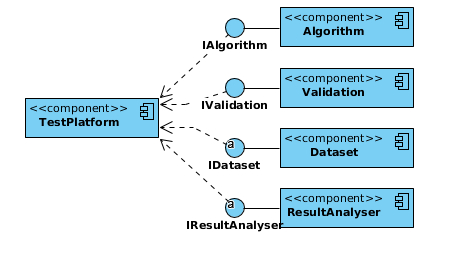
\includegraphics[width=0.9\textwidth]{img/ModulesDiagram.jpg}
	\caption{Schemat modułów systemu.}
	\label{fig:modules_diagram}
\end{figure}

Komponenty są zorganizowane w architekturę wtyczek, omówioną dokładniej w \cite{clean-arch}. Komponenty Dataset, Validation, Algorithm, ResultAnalyser są wtyczkami do TestPlatform. Pozwala to na uniezależnienie komponentów od siebie. Wprowadzanie zmian w logice jednego z komponentów nie będzie powodowało konieczności zmiany zachowania bądź rekompilacji innego komponentu. Dodatkową zaletą może być osobny deployment, niezależnie od przyjętego modelu wdrożenia. Framework będzie wdrażany jako monolityczna aplikacja, ale architektura aplikacji pozwala na łatwe rozdzielenie komponentów na osobne usługi, które mogą być uruchamiane na osobnych maszynach w celu zrównoleglenia obliczeń. Jest to szczególnie ważna cecha istotna w przypadku algorytmów wymagających dużych nakładów mocy obliczeniowej, gdzie równoległe przeprowadzanie obliczeń jest bardzo istotne. Schemat komponentów został przedstawiony na rys. \ref{fig:modules_diagram}.

\subsection{Komponent TestPlatform}

TestPlatform jest odpowiedzialny za konfiguracje eksperymentu, stworzenie wszystkich niezbędnych obiektów i zapewnienie odpowiedniego przepływu danych. Jest to główny komponent, będący punktem wejścia dla użytkownika. Główna logika aplikacji została zawarta w tym komponencie. Pozostałe komponenty zostały oddzielone przez interfejsy. 

\begin{figure}
\centering
	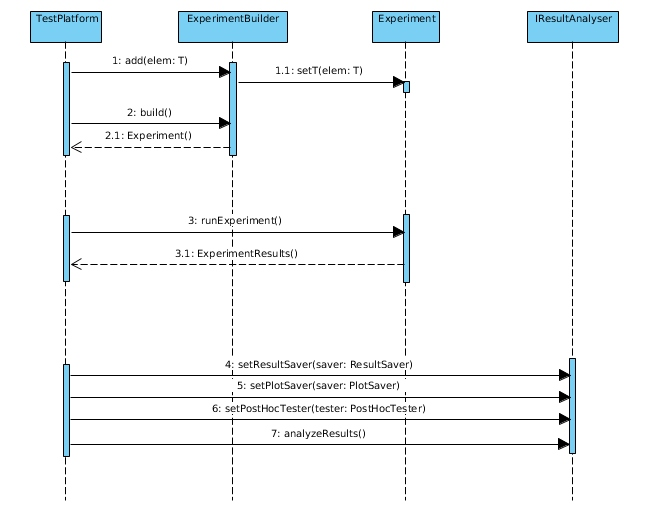
\includegraphics[width=0.9\textwidth]{img/GeneralFlow.jpg}
	\caption{Diagram przepływu w komponecie TestPlatform.}
	\label{fig:modules_diagram}
\end{figure}

\subsection{Komponent Dataset}

Dataset odpowiada za nałożenie abstrakcji na zbiory uczące i pozwala na przeprowadzenie analizy zbioru. 

\subsection{Komponent Validation}

Głównymi odpowiedzialnościami komponentu są podział datasetu na zbiory uczące i testowe o odpowiedniej liczności według przyjętej strategii. Dodatkowo Validation ma dla wygenerowanych zbiorów testowych i uczących zebrać wyniki osiągane przez algorytm. Wyniki te są wykorzystywane w dalszych etapach eksperymentu, ale komponent Validation jest niezależny od dalej zdefiniowanych operacji.

\subsection{Komponent Algorithm}

Komponent jest abstrakcją nałożoną na pojedynczy algorytm uczenia maszynowego, bądź zbiór algorytmów. W zależności od rozwiązywanego zadania (klasyfikacja bądź regresja) wynik działania algorytmu może być różny, tak samo jak przebieg procesu uczenia. Dodatkowo komponent ten przez zastosowanie wzorca projektowego Adapter pozwala uniezależnić implementację algorytmu w wybranych frameworkach uczenia maszynowego od omawianej platformy do testów. 

\subsection{Komponent ResultAnalyser}

ResultAnalyser ma zapisywać rezultaty eksperymentu, generować i zapisywać wykresy oraz przeprowadzać testy statystyczne na podstawie uzyskanych wyników. 

\subsection{Projekt API frameworku}

Projektując framework można skorzystać z dwóch podejść: down-up i top-down. Pierwsze podejście polega na skupieniu się najpierw na zagadnieniach domenowych a następnie budowaniu abstrakcji, które zostają udostępnione użytkownikowi. Drugie podejście polega na zaprojektowaniu interfejsu dla użytkownika w pierwszej kolejności, przechodząc do projektowania i implementacji właściwych mechanizmów w późniejszej kolejności. W projekcie wykorzystano podejście down-up. Oba podejścia mają swoje wady i zalety, niemniej jednak projekt API frameworku definiuje sposób, w jaki ostateczny użytkownik będzie korzystał z naszego kodu. Pomimo przyjętej metodyki projektowania jest to bardzo ważne zagadnienie, które nie może zostać zaniedbane. 

TBD

\section{Kwestie implementacyjne}
%6. Kwestie implementacyjne Na tym etapie zastanawiamy nad wyborem języków implementacji, środowisk i narzędzi.

Obecnie istnieje wiele popularnych obiektowych języków programowania. W niniejszej sekcji pracy przeprowadzono dyskusję możliwych języków implementacji.

\subsection{Wybór języka implementacji}

Język implementacji ma bardzo duży wpływ na ostateczny kształt projektu. Poniżej przedstawiono szczegółową analizę możliwych języków implementacji, wraz z omówieniem zalet i wad wykorzystania wybranych języków do realizacji projektu.

\paragraph{Python}
Python jest językiem typowanym dynamicznie, kompilowanym do kodu bajtowego maszyny wirtualnej. Zyskał dużą popularność przez prostotę składni, przystępność oraz dużą liczbę dostępnych bibliotek. W kontekście realizowanego projektu Python może być wskazanym językiem ze względu na dużą dostępność narzędzi i bibliotek przeznaczonych do uczenia maszynowego. W teorii Python wspiera obiektowość, jednakże pewne mechanizmy związane z dynamicznym typowaniem uniemożliwiają pełne wykorzystanie zasad paradygmatu obiektowego. Przykładowo Python udostępnia możliwość tworzenia interfejsów z wykorzystaniem AbstractBaseClass (ABC). W ABC można zdefiniować metody interfejsu, które muszą być zaimplementowane w klasach dziedziczących po ABC. Brak implementacji skutkuje pojawieniem się wyjątku. Trudno jest zaimplementować zachowania polimorficzne, ze względu na ducktyping. Dodatkowo mechanizm enkapsulacji w tym języku nie istnieje. Jest on symulowany przez name mangling - mechanizm zamiany przez interpreter nazw metod z podwójnym podkreślinikiem na początku nazwy. Istnieją pewne zaawansowane mechanizmy takie jak metaklasy pozwalające na stosowanie refleksji oraz elementy paradygmatu funkcyjnego, które mają wpływ na sposób implementacji w Pythonie, jednakże są mało istotne w kontekście omawianego projektu.

\paragraph{C++}
C++ jest językiem ogólnego przeznaczenia wspierającym wiele paradygmatów. Jego główną zaletą jest szybkość kodu, wynikająca głównie z kompilacji do kodu maszynowego. C++ jest silnie typowany, przez co wiele błędów można wykryć na etapie kompilacji kodu. Niewątpliwą zaletą tego języka jest rozbudowany system szablonów, który pozwala na wykorzystanie zaawansowanych technik metaprogramowania. W \cite{Cpp_turing_complete} wykazano, że szablony C++ są kompletne w sensie Turinga. Oznacza to, że można w nich zaimplementować dowolny algorytm z klasy obliczeniowej rozwiązywalnej na maszynie Turinga. Ciekawym projektem jest \cite{Cpp_snake_compile_time}, gdzie zaimplementowano popularną grę Snake z wykorzystaniem szablonów. Polecenia ruchu są zadawane w czasie kompilacji i jednocześnie w trakcie kompilacji są dokonywane wszystkie obliczenia. Restrykcyjność języka może być powodem wolniejszego tempa implementacji w C++. Dodatkowo operacje na zasobach są jedną z najbardziej niebezpiecznych aspektów tego języka. C++ nie posiada garbage collectora, przez co na programiście ciąży obowiązek zwalniania zaalokowanych zasobów. Istnieją w C++ mechanizmy umożliwiające bezpieczne zarządzanie zasobami, jednakże ich stosowanie wymaga dużego nakładu dyscypliny (przykładowo według Scotta Mayersa najważniejszym wynalazkiem języka jest destruktor, który umożliwił pojawienie się idiomu RAII). Pojawienie się nowszych standardów znacząco poprawiło wygodę programistów i bezpieczeństwo operowania na zasobach, przez np. dodanie inteligentnych wskaźników.

\paragraph{Java}
Java to język w pełni obiektowy, kompilowany do kodu bajtowego. Pełna obiektowość języka oznacza konieczność przynależności zmiennych i funkcji do klas. Nie jest możliwe zadeklarowanie osobnych zmiennych jak to jest możliwe np. w C++. Maszyna wirtualna Javy posiada wiele mechanizmów pozwalających na zwiększenie efektywności programów, takich jak JIT compiler, przez co Java zyskała na popularności w aplikacjach działających po stronie serwera. Dodatkowo wykorzystanie grabage collectora pozwala zmniejsza odpowiedzialność programisty, co przyczynia się do zwiększenia popularności języka.

\paragraph{C\#}
C\# jest podobnie jak Java językiem czysto obiektowym kompilowanym w pierwszym etapie do kodu pośredniego (IL - intermediate language), a następnie do kodu maszynowego za pomocą kompilatora JIT. C\# jest oparty na frameworku .NET.

\subsection{Wybór środowisk i narzędzi}

TBD

\section{Podsumowanie i dyskusja krytyczna}
%7. Podsumowanie i dyskusja krytyczna Tu zamieszczamy spostrzeżenia na temat wykorzystania w projekcie ciekawych technik i co dzięki nim zyskaliśmy.

Zweryfikowano poprawność przygotowanej architektury poprzez sprawdzenie zgodności z zasadami SOLID. Istnieją pewne odstępstwa od tych zasad, ale są one świadomymi kompromisami mającymi na celu uproszczenie projektu (np. podwójna odpowiedzialność klas implementujących IValidationStrategy w komponencie Validation). Nadmierne komplikowanie projektów (ang. overengineering) jest równie poważnym problemem co zbyt prymitywna architektura. Oba te zagadnienia utrudniają rozwijanie aplikacji.

Zastosowanie architektury z podziałem na osobne komponenty oddzielone interfejsami pozwoliło na mockowanie niezaimplementowanych komponentów i niezależny rozwój pozostałych. Jest to bardzo wygodny sposób pracy, umożliwiający prostsze testowanie aplikacji.

\bibliography{bibliography}

\listoffigures


\end{document}